\textbf{Пример 1}
Рассмотрим следующий вызов:

\begin{verbatim}
min_distance([0, 3, 5, 7, 10, 12, 14],
             [8, 7, 9, 7, 6, 6, 9],
             [0, 0, 0, 2, 2, 3, 4],
             [1, 2, 6, 3, 6, 4, 6],
             [1, 6, 8, 1, 7, 2, 5],
             1, 5)
\end{verbatim}

Правильный ответ равен $27$.

Рисунок ниже соответствует \texttt{Примеру 1}:

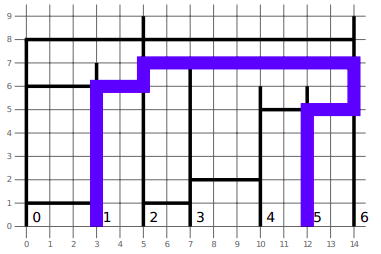
\includegraphics{1.png}

\textbf{Пример 2}

\begin{verbatim}
min_distance([0, 4, 5, 6, 9],
             [6, 6, 6, 6, 6],
             [3, 1, 0],
             [4, 3, 2],
             [1, 3, 6],
             0, 4)
\end{verbatim}

Правильный ответ равен $21$.